\documentclass[10pt]{article}
\usepackage{graphicx}
\usepackage{amssymb}
\usepackage{epstopdf}
\usepackage[]{epsfig}
\DeclareGraphicsRule{.tif}{png}{.png}{`convert #1 `basename #1 .tif`.png}

\textwidth = 7.0 in
\textheight = 9.5 in
\oddsidemargin = -0.25 in
\evensidemargin = 0.0 in
\topmargin = 0.0 in
\headheight = 0.0 in
\headsep = 0.0 in
\parskip = 0.05in
\parindent = 0.0in

\def \fdc    {{\textsc{fdc}}}

\begin{document}

%
% - insert appropriate gluex number here:
%
\title{\scshape{Chapter 15\\ 12 GeV Technical Design Report}\\*[0.5cm]
\upshape{Summaries of GlueX Detector Systems} \\
% Optional Version Number \\
\small{GlueX-doc-323} \\
}
%
\date{Updated: 29 April 2005}
%
% \author{The GlueX Collaboration}
%

\maketitle
%
%
\paragraph{Background}
The goal of the GlueX experiment is to search for gluonic excitations
with masses up to $2.5$~GeV.  The identification of such states
requires knowledge about their production mechanism, the
identification of their quantum numbers $J^{PC}$ and their decay
modes. The production mechanism and $J^{PC}$ determination require a
partial wave analysis which in turn depends on the kinematic
identification of exclusive reactions. The decay products of produced
mesons must be identified and measured with good resolution and with
full acceptance in decay angles.  In many cases the decays of mesons
involve a chain of particle decays.  The GlueX detector (see
Figure~\ref{fig:ch6-hd_schematic}) must therefore be hermetic with 
$4\pi$ coverage and have the capability of measuring directions and
energies of photons and momenta of charged particles with good 
resolution.  Particle identification is also required.


\begin{figure}[t]
\centering
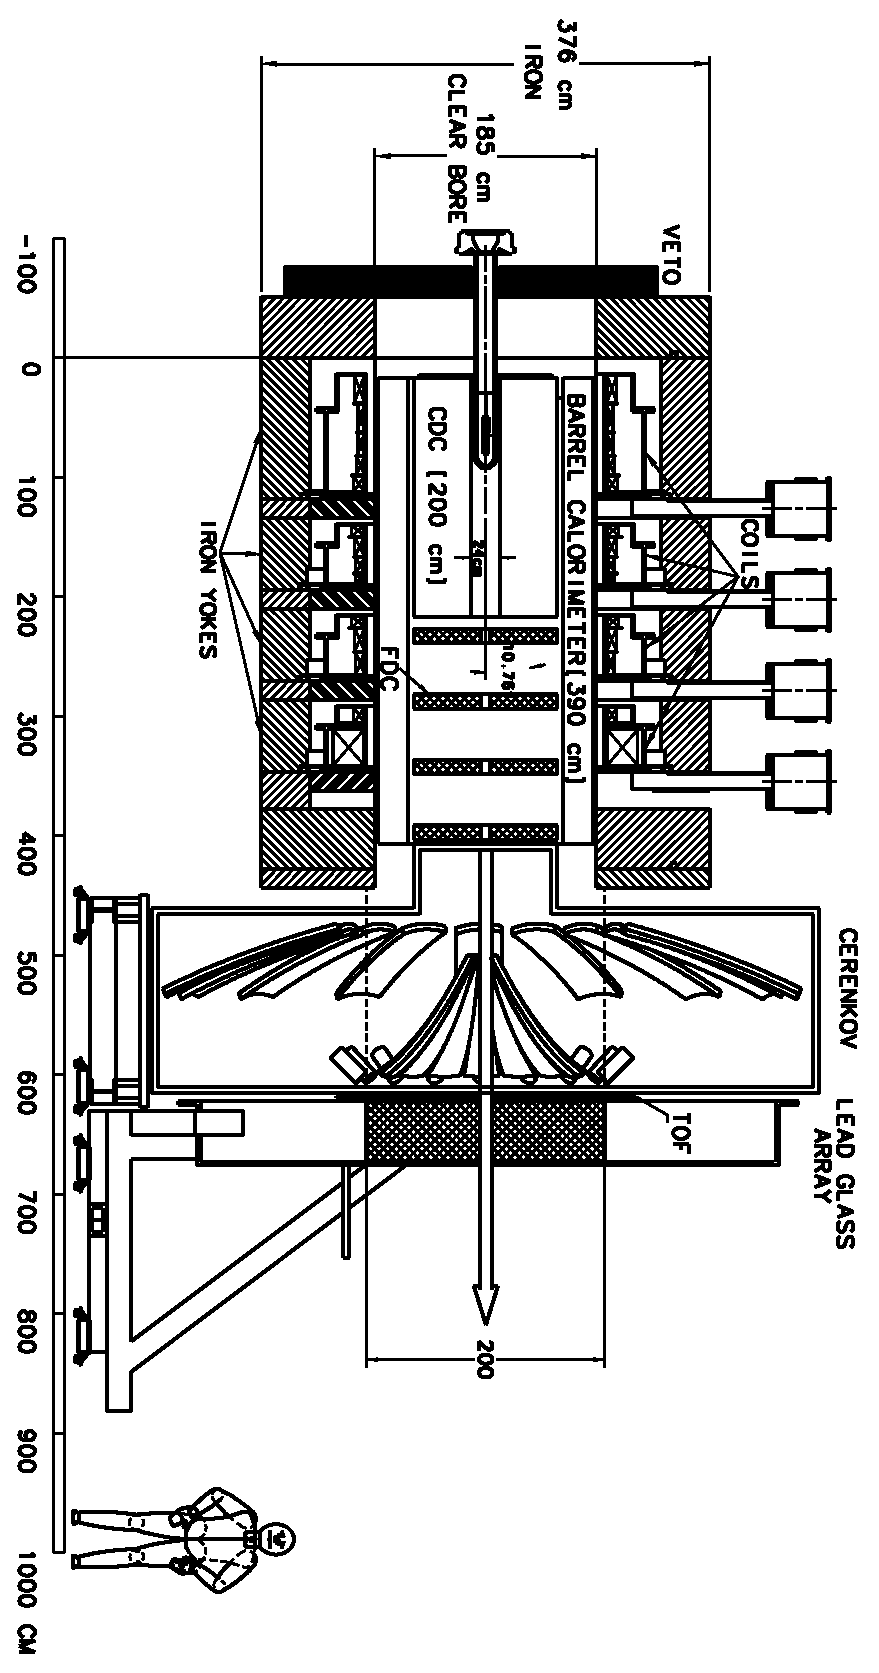
\includegraphics[width=0.50\textwidth,angle=90]{ch6_gluex_detector.eps}
\caption[An overview of the GlueX detector.]{\label{fig:ch6-hd_schematic}
An overview of the GlueX detector. The major subsystems are labeled and 
are summarized individually in the pages that follow. }
\end{figure}

\hspace{1cm}
The partial wave analysis technique  depends on high statistics and
in the case of incident photons, also requires linear polarization.
The latter is needed to identify the production mechanism. The linear 
polarization is achieved by the coherent bremsstrahlung technique.  
The degree of linear polarization and flux of photons in the coherent 
peak fall dramatically as the photon energy approaches
the endpoint energy.  On the other hand, it is desirable to have
photon energies high enough to produce the required masses with
sufficient cross section and with sufficient forward boost for good
acceptance. For a fixed incident momentum and a fixed resonance
mass, it is also desirable to have a fairly constant $\mid t\mid_{min}$ over
the natural width of the resonance.  This also requires sufficiently
high incident photon energy. 

\hspace{1cm}
An operating photon energy $9.0$ GeV produced from a $12.0$ GeV 
electron beam represents an optimization of beam flux, cross--section and 
degree of polarization.  The GlueX detector is therefore optimized for 
this energy range. Figure~\ref{fig:ch6-hd_schematic} is a schematic 
representation of the proposed GlueX detector. The individual 
subsystems are discussed in more detail below.


\paragraph{Hall~D and the GlueX Experiment}

The GlueX experiment will be housed in a new above-ground experimental hall
(Hall~D) located at the east end of the CEBAF north linac. A collimated beam 
of linearly polarized photons (with 40\% polarization) of energy 8.5 to 9~GeV 
will be produced via coherent bremsstrahlung from 12~GeV electrons. This 
requires thin diamond  crystal radiators (no more than 20~$\mu$m thick). 
The scattered electron from the bremsstrahlung will be tagged with sufficient 
precision to reconstruct the photon energy to within 0.1\%.


\hspace{1cm}
The GlueX detector uses an existing 2.25~T 
superconducting solenoid that is currently being refurbished.  An existing 
3000-element lead-glass electromagnetic calorimeter will be reconfigured 
to match the downstream aperture of the solenoid. The collaboration is
currently looking at a DIRC design based on the SLAC BaBar detector for the
Cerenkov system. Design work is being carried out with consultation 
with experts from SLAC. The DIRC Cherenkov Counter is followed by a scintillator 
time-of-flight (TOF) wall which in turn is followed by a lead glass 
calorimeter for detecting photons.  Inside the full length of the solenoid,
a lead and scintillating fiber electromagnetic calorimeter will provide 
position and energy measurement for photons and TOF information for charged 
particles.  A simple start counter will surround the $30\, cm$ long liquid hydrogen
target. This in turn will be surrounded by a cylindrical straw-tube drift-chambers 
which will fill the region between the target and the cylindrical calorimeter.  
Planar drift chambers will be placed inside the solenoid downstream of the target
to provide accurate track reconstruction for charged particles going in the 
forward direction.


\hspace{1cm}
This detector configuration has $4 \pi$ hermeticity and momentum/energy and
position information for charged particles and photons produced from 
incoming $9\, GeV$ photons. This detector has been carefully optimized to 
carry out partial wave analysis of many particle final states.  Extensive Monte 
Carlo studies for a wide variety of final states have been carried out to 
certify the design parameters and the suitability of the detector for carrying 
out the final analysis. In particular, the acceptance of the detector for
final state particles is typically above 95\% and is quite uniform over 
the detector. A well understood acceptance is crucial to being able to carry
out precision partial wave analysis. 


\hspace{1cm}
An active program of R\&D has been underway now for several years on each of the 
detector subsystems. Rocking curve measurements of diamond wafers have 
been performed  in the UK, and the coherent bremsstrahlung technique has been 
successfully demonstrated in Hall~B at Jefferson Lab. Prototypes of tracking 
elements and the cylindrical calorimeter have been built and more are planned.  
Beam tests in Russia on TOF prototypes have resulted in a final design.  
Prototype flash ADCs have been built and tested as have TDCs based on F1 chips.  
Work on optimizing electronics continues and more beam tests are planned.  
The magnet is currently being refurbished at the Indiana University Cyclotron 
Facility. 

\hspace{1cm}
The GlueX detector has undergone several reviews carried out by experts from
outside the JLab community. The electronics was reviewed in the summer of
2003, while the entire detector was carefully looked at in the Fall of 2004.
Finally, a a review was performed on the refurbished magnet. All of these
reviews have led to both improvements and optimizations of the GlueX
detector. The primary characteristics of the detector are summarized in 
Table~\ref{tab:gluex_det}.  The hermetic design for the detector makes it 
an ideal tool to determine the masses and quantum numbers of mesons in the 
mass range of $1.5$ to $2.5\, GeV/c^{2}$. The detector will be sensitive 
to hybrid mesons produced with cross sections as low as a few percent
of well known mesons and can also be used to map out both normal mesons and
the poorly known spectra of $s\overline{s}$ mesons.

\hspace{1cm}
\paragraph{Summaries} This document provides a set of one-page summaries for each of the 
major systems in the GlueX detector. These are not meant to be
detailed, complete discussions, but rather a quick overview of the
entire detector. These summaries briefly outline the 
purpose of the system, the requirements placed on the system by
physics goals of GlueX, and a brief description including channel 
count. This continues with  a discussion of the expected raw signals 
as well as needed amplification and final readout of the detector.
A brief discussion of the current stage of R\&D is given with 
outstanding questions pointed out. Finally, the groups and manpower
needed for final construction of the element are identified as 
well as an estimate of the required construction time. 


\hspace{1cm}
It should be pointed out that due to the availability of both manpower
and interest within the collaboration, some systems are much further
along than others. In particular, the Lead-glass Calorimeter is
being built out of glass blocks from an existing device and a great
deal of experience exists. The Forward Drift Chambers were taken on
by the Ohio University group in late 2002, while the collaboration is
currently in discussions with the University of Tennessee and Oak
Ridge groups about taking responsibility for the Cherenkov system.
Independent of this, the collaboration believes that assuming timely
funding of the detector, a viable plan exists for getting physics 
out of the detector in a timely fashion. 

\bigskip
%\hspace{1cm}
Complete information about the physics goals and description of the GlueX detector
can be found at
\begin{verbatim} 
   http://www.halld.org/cdr_v5/index.html.
\end{verbatim}


\begin{table}[t]
\begin{center}
%\scriptsize
\begin{tabular}{ll}
\hline\hline
{\centering \textbf{\textit{Parameter}}} & 
{\centering \textbf{\textit{GlueX Performance}}} \\
\hline
\multicolumn{2}{c}{\textbf{Charged Particle Detection}} \\
Coverage              & $1^{\circ} < \theta < 170^{\circ}$  \\
Momentum Resolution   & $\sigma(p)/p=1-2\%$ \\    
Position Resolution:  & $\sigma=150-200\mu m$ \\
dE/dx measurements:   & $20\le \theta \le 140^{\circ}$ \\
BCAL time resolution: & $\sigma(t)=200\, ps$ \\
TOF time resolution:  & $\sigma(t)=60\, ps$ \\
$\pi/K$ Separation (Cerenkov) & $\theta < 14^{\circ}$ \\
\multicolumn{2}{c}{\textbf{Photon Detection}} \\
Energy measurments:   & $2\le \theta \le 120^{\circ}$ \\
Veto:                 & $\theta \geq 120^{\circ}$ \\
BCAL resolution ($E_{\gamma}\geq 20 MeV$):  & $\sigma(E)/E=(2+5/\sqrt{E})$ \\
BCAL resolution ($E_{\gamma}\geq 100 MeV$): & $\sigma(E)/E=(3.6+7.3/\sqrt{E})$ \\
BCAL  position resolution & $\sigma(x)=1\, cm$ \\
LGD  position resolution & $\sigma(x)=1\, cm$ \\
\multicolumn{2}{c}{\textbf{DAQ/Trigger}} \\
Level 1:     & $200 kHz$ \\
Event Rate: & $15 kHz$ to tape \\
Data Rate:   & $100 MB/s$ \\
\multicolumn{2}{c}{\textbf{Electronics}} \\
Fully pipe-lined &  FADCs and TDCs \\
\multicolumn{2}{c}{\textbf{Photon Flux}} \\
Initially: $10^{7} \gamma/s$ & Final: up to $10^{8}\gamma/s$ \\
\hline\hline
\end{tabular}
\caption[]{\label{tab:gluex_det}The GlueX detector is
nearly hermetic for both charged particles and photons. The anticipated 
detector performance is summarized in the table.}
\end{center}
\end{table}



 
\clearpage
\begin{center}\textbf{The Tagger System}\end{center}
\subsubsection*{Purpose, Resolution Requirements, Description, Mass, Channel count}
The purpose of the Tagger system is to provide a flux of $\sim 10^{8}$~Hz
of linearly polarized photons from coherent bremsstrahlung in a thin,
orientated diamond crystal. This is achieved by measuring the energies
of the energy degraded bremsstrahlung electrons in the spectrometer.
The photon energy resolution is required to be less than 0.1\% r.m.s.\
of $E_{0}$ for $E_{\gamma}$ between 70\% and 75\%  of $E_{0}$, which
corresponds to 12~$MeV$ r.m.s. energy resolution for a 12~$GeV$ electron beam. 
The Tagger system consists of a quadrupole and 2 dipole magnets, 
a vacuum chamber and the associated focal plane detectors. The dipoles
are two identical magnets that will be run at 1.5~T.  According to the
present design, the pole shoe surfaces will be part of the vacuum chamber.
The focal plane detector array is located just outside the vacuum chamber.
It consists of a set of 141 fixed scintillation counters spanning the full
energy range from 25\% to 95\% of $E_{0}$ and is required for the alignment
of the diamond. A movable ``microscope'' of 120 narrow channels is required
to measure accurately the photon energies in the energy  range 70 to 75\%
of $E_{0}$.  The total mass of the tagging spectrometer system will be
$\sim$ 90 tons.  

\subsubsection*{Raw Signals, Stages of Amplification, Final readout}

Since individual detectors in the focal plane array will have to count
at rates up to $5\times 10^{6}$~Hz, a plastic scintillator/photomultiplier
combination is appropriate.  The fixed scintillator array consists of
paddles 0.5~cm thick mounted perpendicular to the electron trajectories
which span 0.5\% $E_0$ each in recoil electron energy for a total of 141
counters.  The microscope consists of a rectangular array of square
scintillating fibers connected to clear plastic light guides.  Each
fiber is read out with a silicon photomultiplier device, which provides
excellent gain, rate capability and time resolution.  The signals from
the individual fibers are ganged together to form 120 independent tagger
channels of approximately 0.1~\% $E_0$ each.  The digitization electronics
from the focal plane detectors will be standard.


\subsubsection*{R\&D Issues, Simulations and Other Considerations}
The Glasgow  and Catholic Universities groups have calculated the tagger
optics separately, the results of which can be found in Hall D
note 70\footnote{Optics calculation for the Hall D tagging spectrometer
for a 12 GeV electron beam. G. Yang, January 2004.} and the GlueX/Hall D
Design Report (Nov 2002). The Design Report tagger is different from
the design described above. It has a single long, narrow dipole which is
6.1 m in length and weighs $\sim$ 100 tons. Due to concerns about the
mechanical stiffness, the availability of sufficiently large pieces of
iron of the necessary quality and the availability of suitable
manufacturers, Glasgow  and Jlab investigated the possibility of a
tagger consisting of two identical magnets in series\footnote{Optics
calculation for a two magnet tagged photon spectrometer for GlueX.
G. Yang, July 2004.}.
By  careful positioning of the two magnets it is possible to obtain a
design that is equivalent, and in some respects superior, to a single
magnet configuration. The two magnet design concept was accepted by
the collaboration at the Indiana meeting in May 2004. Glasgow has studied
the design in more detail and has produced drawings of the two magnet
assembly, including a possible vacuum system, which should contain
sufficient details for budget prices to be obtained from potential
manufacturers.
It is also relevant to mention that prior to version 4 of the Design Report, 
Glasgow and Jlab investigated the feasibility of a tagger with superconducting 
coils\footnote{Possible designs for a 12 GeV superconducting Tagger. J. Kellie, 
November 2001.} with a magnetic field of 5T and main beam bend angles of 15, 30 
and 45 degrees, for both curved and straight output edges - the room temperature 
tagger bend is 13.4 degrees. After careful consideration, the superconducting 
option was rejected since there are several distinct disadvantages and no 
clear advantages.

\subsubsection*{Manpower, R\&D and Production Schedules}

The Tagger system has been the responsibility of groups from Glasgow 
University, JLab  and Catholic and Connecticut Universities.  More 
work is required to investigate alternative vacuum system designs,
of which several have already been considered. 
%-we have already considered a vacuum chamber which, (i) is external 
%to the tagger dipole magnets, or (ii) uses the pole shoe surfaces as 
%an integral part of the chamber. Vacuum systems which are either 
%completely welded or use a combination of O-ring seals and welds 
%have also been examined.  
It should be realistic to obtain cost 
estimates for the magnets and vacuum system in the near future. 
The Moscow group using ISTC financing could provide the necessary 
manufacturing skill and manpower to produce the magnets and the 
vacuum chamber.  Basic R\&D is required for the focal plane 
assembly, and a decision on which group or groups should take 
on this responsibility should be made in the near future, 
bearing in mind manpower requirements.

\clearpage
\begin{center}\textbf{The Superconducting Solenoid}\end{center}
\subsubsection*{Purpose and Requirements}

The Solenoid is the magnetic element selected for the GLueX Experiment to
provide momentum analysis in the tracking chambers. The Solenoid
is a 73-inch warm bore super conducting (SC) device that produces
a nominal maximum central field of 2.2 Tesla at 1800 Amps. The Magnet is
195 inches long and weighs  approximately 300 tons. The Solenoid was originally
 designed in 1970 as the LASS spectrometer at
SLAC and was subsequently used as the MEGA spectrometer at LANL. The
Solenoid was mothballed in place
in 1995 and first inspected by JLAB Hall D in 2000. The solenoid was
designed as a highly reliable cryogenically stablized SC magnet.
The typical field quality of the solenoid (dB/B $\approx$ 1 \%) is consistent with GlueX
requirements for momentum resolution. The Solenoid was
designed with a slotted yoke and four separate cryostats to accomodate 
the large planar wire chambers used at LASS.
The specific magnetic geometry of the original solenoid had the unfortunate 
side effect of
creating large external magnetic fields, particularly in regions where
phototubes would likely be present. Many of the Solenoid's systems were
inconsistent with JLab operations due either to design or obsolescence; 
the Solenoid had a history
of internal leaks and electrical shorts and had accumulated a substantial 
amount of wear and tear during its 30 year history.
Despite these problems, the robust design and the good state of
preservation made the selection of this solenoid a cost effective
choice for Hall D, even after the necessary costs of modernization and
maintenance were taken into consideration.

\subsubsection*{Status of Upgrading, Modernization and Repair.}

 The first task
performed after the initial evaluation of the Solenoid was to redesign the
yoke magnetic geometry to match the Solenoid to the requirements of Hall D
and to reduce substantially the external fields. The proposed modifications
entail filling the yoke slots and adding steel at the end to reduce yoke
saturation and the escape of internal fields, thus reducing the external
fields by creating a symmetric yoke with a large upstream opening. This
modification also changed the solenoid to a clear bore from end to end.

The MEGA Solenoid was dismantled and shipped to IUCF where it has been 
undergoing some long needed maintenance and repairs. Two of the four
coils are now finished. Refurbishment included repairing LN2 leaks in three coils and a leak
in the LHe vessel of the forth. The shield thermometry is being upgraded to
modern PT-102 Pt resistance thermometers, and the coil support
strain gauges and the deteriorated multi layer super insulation are all being replaced.
The two completed coils were cooled down with
LN2 in July 2004 to perform a final cold leak test and they were
determined to be leak-free to the highest industry standards. This cold testing also 
confirmed that the new instrumentation and insulation worked as designed. 

A mid-course assessment of the solenoid by external experts was held in December of 2004 to
provide advice and recomendations on the present course of restoration and future 
plans for the solenoid. The most significant recomendation was to consider actions 
to eliminate the coil shorts. This advice was taken to heart and a plan was 
concieved to perform a surgical short repair on coil 3 which has a  
hard short to ground. This extra work was incorporated into the work plan for coil 3,
and work on coils 3 and 4 is due to be completed by March 2006.

New Solenoid systems are planned that include a new DC power
supply and energy dump system recently purchased from Danfysik for GlueX.
A new cryogenic interface with JLab compatible automatic valves and
connections and a new control and instrumentation package is under design at JLab.

\subsubsection*{Manpower, R\&D and Production Schedules}

The refurbishment of the coils is being performed at IUCF under
the direction of JLab staff, and will continue until complete.
A cost-benefit analysis is underway to determine the ultimate value 
of a full-scale test of the solenoid including the iron yoke 
in advance of the availability of Hall D, possibly at IUCF.
Ultimately the solenod will be installed and thoroughly tested in Hall D 
prior to the installation of the actual GLUEX apparatus. This installation
is one of the schedule drivers for the experiment, and therefore must be 
streamlined to allow prompt assembly of the detector.
\clearpage
\begin{center}\textbf{The Liquid Hydrogen Target}\end{center}
\subsubsection*{Purpose, Resolution Requirements, Description, Mass, Channel Count}
The main physics program for the GlueX experiment will be conducted with a
low-power liquid hydrogen target. The planned target is $30\, cm$ long and
somewhere between $3$ and $6\, cm$ in diameter. Such targets normally 
employ mylar target cells. The mylar cell will be mounted on a metal base 
to provide for liquid entry ports and a reliable means of positioning the 
cell. The beam enters through a thin window mounted on a reentrant tube at 
the base of the cell. The target cell is connected to a condenser located 
upstream of the cell.

\subsubsection*{R\&D Issues, Simulations, Monitoring and Other Considerations}
The maximum power deposited in the target by the beam is $100\, mW$.  In such low-power
targets, natural convection is sufficient to remove heat from the target cell and a
circulation pump is not required. A system such as this, containing a few hundred 
$cm^3$ of liquid hydrogen, would be considered ``small" by Jefferson laboratory standards
and the safety requirements would not place any significant constraints on the target
design or operation.

\subsubsection*{Manpower, R\&D and Production Schedules}
The target will be built by the JLab target group. It is estimated that
approximately one year will be required to design, construct, test and
certify the target. This target is very similar to other targets that
have been built at JLab, partcularly for Hall B.


\clearpage
\begin{center}\textbf{The Start Counter}\end{center}
\subsubsection*{Purpose, Resolution Requirements, Description, Mass, Channel Count}
The start counter is used to provide a start signal for
time of flight measurements and to identify  the beam pulse associated
with the observed event. In order to be independent of particle momenta
and trajectories, the start counter is located as close to the target as
possible. To be able to identify beam pulses the detector
needs a minimal time resolution of 300~ps. 

The detector will consist of an array of 30 to 60 scintillators
cylindrically surrounding the target. The inner diameter of the
cylinder is 10~cm. Each scintillator element will have  
a thickness of 3 to 5~mm and a length between 45~cm and
70~cm. The optimal dimension will be determined from simulation. The
detectors can be read out either via high magnetic field PMT's or
other detection methods based on solid state detectors.     

\subsubsection*{Raw Signals, Stages of Amplification, Final Readout}
From studies using cosmic rays we have determined that high field
PMT's such as the Hamamatsu R5942 (H6614-01 system) can provide a time
resolution of 250~ps which makes is suitable for our application. For
minimum ionizing particles we obtained signal sizes of about 0.4~V
with a rise time of about 5-8~ns.

\subsubsection*{R\&D Issues, Simulations, Monitoring and Other Considerations}
The timing performance of the Hamamatsu tube must be determined in
various magnetic field configurations. Other readout methods including
VLPC and SiPM will also be studied to investigate the feasibility of a
double ended readout system. Further simulations are needed to finalize
the detector geometry.

\subsubsection*{Collaboration Responsibilities}
FIU is responsible for the start counter. In its current form, without
the need of high resolution position information, the available man
power at FIU is sufficient.
We expect that the counter can be built on the time scale of two years.




\clearpage
\begin{center}\textbf{The Straw-tube Chamber}\end{center}
\subsubsection*{Purpose, Resolution Requirements, Description, Mass, Channel count}

The purpose of the CDC is to accurately measure $(r,\phi,z)$
coordinates along charged-particle tracks. In conjunction with the FDC, it
will then  reconstruct the momentum, $\vec{p}$ of each track and the primary and
secondary vertices's of the event. The exact momentum resolution is a function 
of particle momentum and the number of hits in both the CDC and FDC. Monte Carlo
studies indicate that an $r\phi$-spatial resolution, $\sigma_{r\phi}$, on the 
order of $150$ to $200\mu m$ is sufficient to satisfy the physics goals of the 
experiment. The $z$-coordinate is obtained using $6^{\circ}$ stereo layers. 
The resolution is given as $\sigma_{z}=\sigma_{r\phi}/\sin 6^{\circ}$.  
The CDC also needs to provide $dE/dx$ information sufficient for separating 
$K$s and $\pi$s for particle momentum under $0.500\,GeV/c$.

The chamber is built using 23 layers of $1.6\,cm$ diameter, $100\mu$ thick
aluminized kapton, $2\,m$ long straw tubes. The signal is measured using a
$20\mu$ diameter gold-plated tungsten wire strung under $55\, g$ of tension.
Layers $5$, $6$, $14$ and $15$ are $+6^{\circ}$ stereo while layers
$7$, $8$, $16$ and $17$ are $-6^{\circ}$ stereo. Due to the packing of the
tubes, the exact channel count depends on the exact specifications of the
final chamber, but is presently estimated to be $3240$ channels.

\subsubsection*{Raw Signals, Stages of Amplification, Final readout}

A minimum ionizing track produces about $30$ primary ionizations per 
centimeter of traversed gas. Path length in a straw-tube depends on
both the distance away from the wire as well as the polar-angle $\theta$
of the track, but typical values vary between about $0.5\, cm$ to a few $cm$.
The chamber will be run such that the gas amplification is about $10^{4}$.
The signals will be read out using capacitively coupled preamps mounted
directly on the upstream end plate of the detector and then fed into 10+ bit
FADC and digitized at 125~MHz. Due to the $2.25\, T$ magnetic field, the maximum
drift times will be on the order of $800~ns$ for a typical gas mixture. 


\subsubsection*{R\&D Issues, Simulations, Monitoring and Other Considerations}

The group is currently stringing wires in a $\frac{1}{4}$-chamber, full-scale 
prototype. We have currently identified several design changes that will
facilitate easier construction. Apart from construction technique, the main
 issues to be resolved with the prototype are gas distribution and electronic
hook-ups.  


\subsubsection*{Manpower, R\&D and Production Schedules}

The CDC is the responsibility of the Carnegie Mellon University group. Assuming that
a team of stringers is hired during the actual fabrication phase (as has been
done with other chamber projects), the group has sufficient manpower to build the
final device on a time scale of three and a half years from the time that funds
become available. The group expects to work with the FDC team and the JLab electronics
group to build a preamp that is common to all chambers in the experiment.  


\clearpage
\begin{center}\textbf{The Forward Drift Chambers}\end{center}
\subsubsection*{Purpose, Resolution Requirements, Description, Mass, Channel Count}

The \fdc{}s include 4 separate packages of disk-shaped horizontal drift chambers 
to measure the momenta of all charged particles emerging from the target at 
angles of up to 30$^{\circ}$ relative to the photon beam line.  Each package
consists of 6 planes of alternating anode and field-shaping wires with a 
wire-to-wire separation of 5~mm (119 anode wires per plane) and with 150~$\mu$m 
spatial resolution from the drift time readout.  Each wire plane is sandwiched 
between 2 planes of cathode strips (238 strips per plane with 5~mm pitch).  By 
charge interpolation of the electron avalanche image charge in the cathode strip 
readout, spatial resolutions at the cathode planes are expected of better than 
150~$\mu$m.  The strips are arranged in a $U$ and $V$ geometry with respect to 
the wires (at $\pm$45$^{\circ}$) allowing for separation and assignment of 
multiple hits within a chamber to the different tracks.  Adjacent chamber 
elements will be rotated by 60$^{\circ}$ with respect to each other in order 
to improve track reconstruction decisions on the corresponding anode wire 
left/right ambiguities, hence improving the overall resolution.  The wires 
that cross through the beam line will be deadened out to a radius of 3.5~cm 
to reduce the rates.  Each \fdc{} package has a channel count of 3570, leading 
to a total channel count for the full \fdc{} system of 14280 (2856 anodes and
11424 cathodes).

\subsubsection*{Raw Signals, Stages of Amplification, Final Readout}

Each signal from the \fdc{}s (anodes and cathodes) will be sent to a
chamber-mounted charge-sensitive preamplifier that drives a pulse-shaping 
amplifier. The signals from the anode wires that are above some 
pre-determined voltage threshold will be discriminated and then digitized 
by 125~ps LSB resolution F1 TDCs.  The signals from the cathodes will be digitized with 
62.5~MHz 10-bit flash ADCs.

\subsubsection*{R\&D Issues, Simulations, Monitoring and Other Considerations}

The primary development issues that must be addressed for the \fdc{} system
are factors affecting the intrinsic resolution of the chambers, along with 
the mechanical and electronics layout.  The goal is to construct a tracking 
detector that meets the required design specifications and has a long life 
time, a uniform and predictable response, a high efficiency, and is 
serviceable in case of component failure.

Two detector prototypes will be completed and studied over the course
of the next three years.  The first will be employed to study the optimal 
electrode configuration for the system.  A second full-scale prototype
will be completed to test mechanical support designs for the chamber 
cathode planes and wire planes, which is necessary to avoid electrostatic 
instabilities and non-uniformities that are known to affect resolution. 
This second prototype will also be essential to complete the final design 
of the \fdc{} circuit boards.  A significant aspect of the design work includes 
development and study of Monte Carlo of the GlueX detector system focussing 
on the properties of the \fdc{} system that will enable us to meet or exceed 
the required design specifications.

The detector group at Jefferson Laboratory is developing the gas system
for the entire GlueX experiment.  The Ohio University group will work
to ensure that this design is adequate for the control and monitoring
of the \fdc{} system.

\subsubsection*{Collaboration Responsibilities}

The \fdc{} prototyping and design is primarily the responsibility of
the Ohio University group, with important support from the detector
group at Jefferson Laboratory.  The manpower available is adequate
to complete the detector R\&D within 3 years and to complete the
detector construction with 4 years pending availability of funds.


\clearpage
\begin{center}\textbf{The Cherenkov Detector}\end{center}
\subsubsection*{Purpose, Resolution Requirements, Description, Mass, Channel count}

The Cerenkov detector is to serve as part of the particle identification system
together with the time-of-flight system for forward-going charged particles.
The goal is to distinguish between pions, kaons and protons with
momenta above the reach of the time-of-flight system. Here we describe the DIRC,
one of options considered for this task.

The DIRC uses thin, long rectangular bars made of synthetic fused silica
(quartz) both as Cerenkov radiators and light guides  with
an index of refraction of $n \approx 1.47$. The design is based on the
successful novel technique for particle identification developed for
BABAR \footnote{I. Adam \em{et al.} Nucl. Instr. \& Meth. \textbf{A538} 281 (2005).}.
A fraction of the Cerenkov photons produced by relativistic charged particles 
in the quartz bar remain inside the bar due to total internal reflection.
These photons are collected at the end of the bars and imaged onto 
an array of photomultiplier tubes preserving sufficient angular precision to
determine the angle of the produced Cerenkov light. The DIRC can provide 
identification of pions, kaons and protons with an efficiency of better 
than 90\% and a mis-identification rate below 10\% for momenta up to 4.5 GeV/c. 
The current design for GlueX requires 60 quartz bars and 2000 photomultiplier 
tubes.

\subsubsection*{Raw Signals, Stages of Amplification, Final readout}

An electron will create about 30 detected photoelectrons in the struck bar.
The photomultipliers need to be sensitive to single photoelectrons
with sufficient time resolution to minimize out-of-time photons converting
in the quartz. The rate per tube is expected to be approximately 100kHz.
The photomultiplier tubes will be placed at a distance of
about 3 m on one side of the GlueX detector where the fringe fields of 
the solenoid are below 100 G. Efficient shielding of the field can be achieved
with standard techniques.


\subsubsection*{R\&D Issues, Simulations, Monitoring and Other Considerations}

While the principle and hardware of the BaBar DIRC with modifications of 
the geometry are applicable to the GlueX detector we explore possible 
improvements of the imaging. 
The exact exit position of a Cherenkov photon from a bar is unknown.
At BaBar this uncertainty is reduced by placing the phototubes at some
distance to measure the photon direction from the bar. This pinhole focusing
requires a large water tank. On the other hand, focusing of the photons
with mirrors onto multi-channel photon detectors increases the spatial
resolution and allows a compact assembly. Such devices also provide higher
precision in the measurement of the photon arrival time which allows to
correct for the significant smearing of the Cherenkov angle due to the 
unknown photon wavelength. As for the readout we investigate leading-edge 
versus constant-fraction discrimination together with the TDC solution of 
GlueX. A prototype of a focusing DIRC with cylindrical mirrors is currently
being tested at SLAC
\footnote{C. Field \em{et al.} Nucl. Instr. \& Meth. \textbf{A518} 565 (2004).}.
Simulation studies are performed to optimize the mirror imaging and 
the final design.

\subsubsection*{Manpower, R\&D and Production Schedules}

The Cerenkov detector for GlueX is not as well developed as other detector components.
This is due to the fact that the first group to express interest in this detector
is no longer part of the collaboration. After the granting of CD0 to the JLab upgrade,
a pair of groups from Tennessee approached the collaboration and are eager to take
on the responsibility for a major detector. Based on a fresh look at the challenges
for particle identification and their own expertise, they have proposed the
construction of a DIRC detector which is a very good match to particle identification
in this momentum range. A final decision on the detector technology we will use clearly
depends on many factors including physics, manpower, costs and timescales. The collaboration
is currently evaluating all of these. 

\clearpage
%\begin{center}\textbf{The Cherenkov System}\end{center}
%\input{Cherenkov}
%\clearpage
\begin{center}\textbf{The Time-of-flight Wall}\end{center}
\subsubsection*{Purpose, Resolution Requirements, Description, Mass, Channel Count}

The purpose of the TOF is to serve as part of the particle identification system
in conjunction with a Cerenkov detector for forward-going charged particles.  The
goal is to separate $\pi^{\pm}$ from $K^{\pm}$ for momenta up to 2~GeV/$c$ and 
for the given geometry a 95\% separation efficiency is achieved 
at the highest momentum with a time resolution of 80~ps.  The TOF will use
two planes of scintillator bars located immediately upstream of the lead glass
detector (LGD).  Based on simulations and prototype studies the bars will be
250~cm long, 6~cm wide and 1.5~cm thick.  Thus the mass presented by the 
detector immediately before the LGD corresponds to 3~cm of scintillating plastic.
Each bar is read out at both ends with a photomultiplier.  The channel count is 168.

\subsubsection*{Raw Signals, Stages of Amplification, Final Readout}

Prototype studies with a cosmic ray test facility at Indiana U and extensive tests
in a hadron beam at IHEP (Protvino, Russia) included various scintillating bars
of different thickness (1.5~cm, 2.5~cm and 5.0~cm) with various photomultipliers
(Russian FEU-115, Hamamatsu R5506 and R5946, and Philips XP2020).  The
XP2020 was chosen.   The typical pulse has a rise-time of less than 5~ns and
an amplitude of about 0.5~V.  Constant fraction discriminators will be used and 
a TDC with a least count of 25~ps.

\subsubsection*{R\&D Issues, Simulations, Monitoring and Other Considerations}

The performance of the prototype TOF in
a 5~GeV/$c$ hadron beam at IHEP has been described in three NIM 
publications\footnote{Nucl. Instr. \& Meth. \textbf{A478} 440 (2002); 
 Nucl. Instr. \& Meth. \textbf{A494} 495 (2002);
Nucl. Instr. \& Meth. \textbf{A525} 183 (2004) }.  For the 1.5~cm thick TOF bar,
a time resolution for a two-bar system of 77~ps at the bar center and 40~ps
near the ends was achieved.  Magnetic shielding studies were also carried out
and are described in a NIM publication\footnote{Studies of magnetic shielding
for phototubes; accepted and
available online at www.sciencedirect.com 10 Aug 2004}.  Further R\&D measurements
with an array of scintillator bars in a hadron beam at IHEP are planned within the
next year.


\subsubsection*{Collaboration Responsibilities}

The TOF is the responsibility of the groups from Indiana University and the Institute for
High Energy Physics (IHEP) in Protvino, Russia.  This manpower is adequate to complete
remaining R\&D in six months and to complete the detector construction in
two years from availability of funds.


\clearpage
\begin{center}\textbf{The Barrel Calorimeter}\end{center}
\subsubsection*{Purpose, Resolution Requirements, Description, Mass, Channel count}
The purpose of the BCAL is the detection and energy determination
of photons and charged particles from the decays of the neutral
$\pi$, the $\eta$ and other mesons decaying into photons.  All
charged particles that fall within its volume as they are swept
by the magnetic field, mostly in the momentum range of $300-1000\, MeV/c$,
will also be detected.  Some spatial information can also be extracted
from the timing information relative to the two read-out ends of the BCAL.
The design of the BCAL is based on that of the KLOE calorimeter at LNF
in Italy. The expected energy resolution for photons is
$\sigma(E)/E\approx 0.02+0.05/\sqrt{E}$, while the expected timing
resolution is $\sigma(t)\approx 200\,ps$.  The physical layout of the
BCAL is a ring consisting of $48$ modules (segments) at an inner radius
of $65\,cm$ and an outer radius of $90\, cm$.   Thus, its  approximate thickness
is $25\, cm$ corresponding to approximately $18-19$ radiation lengths. The nominal
length of each module is $400\, cm$.  Each module is constructed as a matrix
of $96$ double clad scintillating fiber optic strands (SciFi+IBk-s), embedded
on grooved Pb sheets of $0.5\, mm$ thickness. Thus, each module consists of
approximately $220$ layers of Pb/SciFi and special optical epoxy composite.
The high magnetic field and limited space available for read out, is an
area of particular concern with several emerging technologies, such
as SiPM's, offering the most attractive solutions. Extensive R\&D is still
needed to finalize the type of readout devices and the required channels.


\subsubsection*{Raw Signals, Stages of Amplification, Final readout}
It is clear that a large number of SciFi+IBk-s will be read out by any of the
selected PM's.  The exact number depends on PM window size and its saturation
properties.   Assuming $1\, mm^{2}$ to $3\, mm^{2}$ SiPM window area and a 
$5\,cm \times 5\, cm$ matrix area viewed, approximately $1600$ SciFi's will 
be viewed by a number of SiPM's. The optimum number of SiPM's required will 
depend on the nature and geometry
of the light concentrator and diffuser and the light collection efficiency of
the optical fibers that will transport the light to the SiPM's.   This
requires R\&D and testing of various configurations, however early studies
indicate between a number 10 and 20 SiPM's.  Each group will be coupled to
provide one (fast) analog signal similar to that from vacuum PMT's, which
are thus subject to standard ADC and TDC processing.




\subsubsection*{R\&D Issues, Simulations, Monitoring and Other Considerations}
The R\&D on the actual construction of the BCAL is almost complete with
a full-scale $4$~m module built, and tested with cosmic-rays.  The
read-out requires significant R\&D and MC simulations, more so because the SiPM
technology is still not yet mature and specifications and performance improve
with demand and experience.  This R\&D has already started and most likely will
result in collaboration with DESY, CERN, KLOE and Russian groups to custom
tailor the devices to our needs.  The monitoring system of the read-out devices
can be done by using a pulsed laser-fiber optic combination.



\subsubsection*{Collaboration Responsibilities}

The BCAL is the responsibility of the UofR SPARRO group.   For the construction
of Module 1 and subsequent production modules, as well as radiation damage
studies of the SciFi's, the CSR group at the University of Alberta is also
assisting.  This combined manpower is adequate to complete the R\&D phase
by the end of 2005.   It is also adequate to complete the construction of
the BCAL subject to external funding and adequate construction timelines.
The high-energy physics group at the University of Athens will be assisting
with the SiPM R\&D, as the European component of this emerging technology effort.


\clearpage
\begin{center}\textbf{The Lead-glass Calorimeter}\end{center}
\subsubsection*{Purpose, Resolution Requirements, Description, Mass, Channel Count}

The purpose of the LGD is to detect and measure the energy and position of photons
from the decays of $\pi^0$, $\eta$ and other mesons.  LGD's of similar construction
were used in experiments at Brookhaven (E852 - using a pion beam) and JLab (Radphi
-using a photon beam).  
 The energy resolution
given by $\sigma(E)/E = 0.036 + 0.073/\sqrt{E}$.
Shower positions at the LGD plane
 are reconstructed with a resolution
 of $\sigma_r = \sqrt{(7.1/\sqrt{E})^2 + (X_0 \sin\theta)^2}$~mm
 where $X_0$ is the radiation length of the lead glass
 (30~mm) and $\theta$ is the photon angle measured with respect
 to the normal to the LGD (energies in GeV). This leads to mass resolutions of 10~MeV/$c^2$
 and 30~MeV/$c^2$ for the $\pi^0$ and $\eta$ respectively.
   The detector consists of 2300 lead
glass blocks of dimensions $4 \times 4 \times 45$~cm$^3$ arranged in a nearly circular
stack of radius $\approx$1~m.
  The Cerenkov light from each block is viewed by a FEU-84-3 Russian phototube. 
The phototube bases are of a Cockcroft-Walton (CW) design.  The phototubes are resigtered 
with respect to the glass using a cellular wall that includes soft-iron and $\mu$-metal
shielding. Since the LGD is the furthest downstream subsystem in the overall
GlueX detector, the mass presented to particles is not an issue.  The channel count is 2300.

\subsubsection*{Raw Signals, Stages of Amplification, Final Readout}

A 1~GeV photon produces about 800 photoelectrons corresponding to a phototube
signal of about 0.5~V and a rise-time of 10~ns.  No further amplification is required.  
The signal will be digitized with an 8-bit 250~MHz FADC.

\subsubsection*{R\&D Issues, Simulations, Monitoring and Other Considerations}

The performance of the LGD has been described in two NIM publications for E852 
experiment\footnote{Nucl. Instr. \& Meth. \textbf{A332} 419 (1993); 
 Nucl. Instr. \& Meth. \textbf{A387} 377 (1997)} 
and a a submitted NIM article for Radphi. An earlier version of the CW base is described
in another NIM
publication\footnote{Nucl. Instr. \& Meth. \textbf{A414} 466 (1998)}.  GlueX R\&D has concentrated on
construction of 100 prototype improved CW bases, evaluation of  lead glass and FE-84-3
phototubes used in E852 and Radphi to
determining suitability for use in GlueX and various curing techniques to repair radiation damage of
lead glass.  Simulations of detector response is based on extensive
experience with E852 and Radphi data analysis.  Raphi experience is particularly important
as it involved operating an electromagnetic calorimeter in an bremsstrahlung
photon beam.
The monitoring system consists of a plastic scintillator sheet covering the 
up stream end of the glass stack
and illuminated by fibers connected to a pulsed laser.  



\subsubsection*{Manpower, R\&D and Production Schedules}

The LGD is the responsibility of the groups from Indiana University and the Institute for
High Energy Physics (IHEP) in Protvino, Russia.  This manpower is adequate to complete
remaining R\&D in six months and to complete the detector construction (including CW bases) in
two years from availability of funds.


\clearpage
\begin{center}\textbf{The Upstream Photon Veto}\end{center}
\subsubsection*{Purpose, Resolution Requirements, Description, Mass, Channel count}

The purpose of the UPV is to detect backward going photons of energy greater than 20 MeV 
emerging from the target region. The UPV provides the upstream coverage of the hermetic 
photon detection. The design of the UPV employs a traditional lead-scintillator sampling 
calorimetry.   The detector is able to detect multiple photons with fast detection and 
with timing information that may be utilized at the trigger level.

The UPV consists of 18 layers of scintillator alternating with first 12 layers of lead 
sheets (0.36 radiation length thick) then 6 layers of  lead sheets (0.72 radiation 
length thick). The expected energy resolution for incident photons is 
$\sigma(E)/E = 5\% + 8\%/\sqrt{E}$ at a $24\%$ sampling fraction. Each  scintillator 
layer consists of seven 34cm x 238 cm paddles forming a plane. The central paddle 
has a 10 cm hole to allow for the passage of the beam. The effective area of each 
plane is approximately 238 cm x 238 cm. The total counter thickness is 8.91 
radiation lengths.   The layers are arranged into 3 alternating orientations: 
x, u, and v ( $\pm45^o$, respectively).  


The scintillation light is collected at one end of each paddle only.  For each 
orientation, the light collecting ends of the scintillators are join together 
via a wavelength shifter which is oriented perpendicular to the  scintillators.  
The wavelength shifter is used to redirect the light through $90^o$ and out the 
upstream end of the solenoid to photomultipliers tubes (PMT).  Each PMT is 
protected from fringe magnetic field with soft steel casing and mu-metal shield. 
The channel count is 21.

\subsubsection*{Raw Signals, Stages of Amplification, Final readout}

A typical pulse has a signal of 500 mV and a rise time of 10 nSec corresponding 
to about $10^3$ photoelectrons at $10^7$ PMT gain. The signal will be digitized 
using standard FADC and TDC modules.  

\subsubsection*{R\&D Issues, Simulations, Monitoring and Other Considerations}

Initial R\&D on the construction and building techniques of a prototype module 
is near completion. Measurements of prototype performance in a low energy 
electron beam are planned for later this year.  These results will be compared 
to Geant4 simulations.   R\&D continues on optimizing light collection, 
channel segmentation, and read-out. SiPM's, an emerging technology which is 
being studied for use in the BCAL, offer an attractive read-out solution 
along with potential benefits in light collection and in minimizing high 
magnetic field effects. The monitoring system of the UPV read-out can be 
tied into the system utilized for the BCAL detector, which uses a pulsed 
laser-fiber optic system.



\subsubsection*{Collaboration Responsibilities}

The UPV is the responsibility of the group from Florida State University.  
This manpower is adequate to complete remaining R\&D and to complete the 
detector construction in two years from availability of funds.


\clearpage
\begin{center}\textbf{Electronics}\end{center}
\subsubsection*{Purpose, Description}

The electronics will amplify, discriminate, and digitize raw detector signals
storing them for later readout at level 1 trigger rates of 200 kHz
without incurring deadtime.  The detector includes
approximately 18,600 ADC channels and 6,300 TDC channels.

A pipelined approach is required due to the high trigger rate.  The
digitized information must be stored for several $ \mu s $ while the
level 1 trigger is formed.  Multiple events must be buffered within
the digitizer modules and read or transmitted while the front ends continue to
acquire new events.  The raw data rate from the detector is about 1
Gbyte/second. A sophisticated timing system is required to synchronize the
pipelines in the front-end modules.  The plan is to clock all digitizers in synchronization
with the accelerator timing.

Energy sums from the calorimeters as well as track counts from the barrel and TOF systems
compromise the level 1 trigger.



\subsubsection*{Current Status, R\&D issues}


Since no currently available commercial solutions exist the 
preamps, discriminators, digitizer modules, and timing system
will be designed by GlueX.

JLab has designed a multi-channel TDC module based on the ACAM TDC-F1
chip, and 100 units are currently in use in existing JLab experiments.  A high density
FADC with auxiliary user-definable processing is currently being developed at
Jefferson Lab.

A single-channel prototype 8-bit 250~MHz FADC, suitable for the barrel
and lead glass calorimeters, has been constructed at Indiana
University.  A multi-channel version which includes the energy sum is
currently being designed.

 A prototype constant-fraction discriminator has been built at the University of Alberta.

Preliminary work has been done on the preamps and
the timing system, and on a slower FADC for the tracking chambers.




\subsubsection*{Review}

The GlueX electronics system was reviewed in July of 2003.  The
reviewers concluded the basic design is sound and appropriate assuming
adequate human and fiscal resources.

The reviewers recommended that the work on the TDC and FADC should
continue.  A multi-channel FADC needs to be prototyped and evaluated.
As part of the level-1 trigger, the digitized calorimeter signals are
summed in a pipelined adder tree; the prototype FADC needs to
demonstrate this capability.

Analog front-end requirements need to be settled.  Prototype work
needs to begin, especially on the tracking chamber electronics to be
located inside the magnet.  The pipelined level-1 trigger, timing,
synchronization, and calibration systems all need further development.



\subsubsection*{Manpower, Management, and Schedule}

The reviewers concluded that current manpower resources are
inadequate.  The University of Alberta has recently joined the
collaboration, but additional institutions possessing electronics
expertise are needed.  Discussions are under way with the Indiana University
Cyclotron Facility.

The reviewers concluded that a rudimentary management plan exists, but
that it needs further development.  

The reviewers estimated that the GlueX electronics effort could
require 6 years to complete after CD-3; the collaboration hopes to
reduce this time.  One possibility is a commercial partner/collaborator.

\clearpage
\begin{center}\textbf{Data Acquisition}\end{center}
\subsubsection*{Purpose, Description}

The data acquisition system must:
\begin{itemize}
\item support a deadtimeless front-end system at a 200 kHz trigger rate
\item collect data from the front-end modules at 1 GB/s
\item build event fragments into a single event record
\item pass built events to a level 3 farm
\item write level 3 accepted events to mass storage at 100 MB/sec
\item deliver a small subset of the events to calibration and
  monitoring systems
\end{itemize}

GlueX expects to fill approximately 70 readout crates 
containing 25,000 channels of electronics. 
We expect a level 3 reduction of 90\%, which reduces the 1 GB/s raw
rate to an accepted event data rate of 100 MB/s.

\subsubsection*{Current Status, R\&D issues}

GlueX will use CODA, the standard DAQ system developed at JLab, but at
higher trigger and data rates than have been achieved so far.  We note
that the high rate makes it impossible to interrupt the front-end
processors for every event, parallel event building will be required,
and that CODA has not been run with a high-rate level 3 farm.

CODA is under active development by the DAQ group at JLab.



\subsubsection*{Manpower, Further R\&D, Production}

Primary responsibility for developing CODA belongs to the DAQ group at
JLab.  This includes all the software needed to  
program and collect data from the front-end boards,
build events,
deliver and analyze events in a level 3 farm,
and write events to local mass storage.
The JLab computer center is responsible for moving the data (100
MB/s) from local mass storage to permanent storage at the central
computing facility.

Note that the DAQ group will develop the software infrastructure
required to run the level 3 farm, while GlueX will build and run the
farm, and develop the level 3 trigger algorithm.  We further note that
the DAQ group must be intimately involved with the GlueX electronics,
trigger, and online efforts.

A prototype DAQ system needs to be available two to three years before
start of data taking, and the production system must be ready one year
before the start of data taking.


\clearpage
\begin{center}\textbf{The Online System}\end{center}
\subsubsection*{Purpose, Description}

The online effort is the umbrella under which all efforts related to
taking data and writing it to mass storage will be organized, and
includes overall responsibility for designing, installing, and
maintaining everything related to controlling and running the
experiment.  This effort covers
\begin{itemize}
\item electronics and trigger installation
\item experiment network design and installation
\item counting house and operator environment
\item DAQ installation and customization
\item run management and control
\item construction and maintenance of level 3 farm
\item online event monitoring 
\item online event display
\item electronic logs and bookkeeping
\item slow controls
\item alarm systems
\item online calibration farm
\end{itemize}


\subsubsection*{Current Status, R\&D issues}

Most of the R\&D needed here is being done by other groups, especially
the Electronics, DAQ, and Trigger groups.  For the remainder we will
adapt existing or soon to exist technology (from JLab, CERN, Fermilab,
SLAC, industry, etc.) as needed.  The main effort will go into
customizing the chosen technologies and integrating them into a
coherent and usable online system.



\subsubsection*{Manpower, Further R\&D, Production}

GlueX will take primary responsibility for the online effort, and we
expect that a large fraction of the work will be done by experimenters
residing at JLab.  The online software effort is substantial,
involving customization and integration of a wide variety of outside
packages.  The online hardware effort is also substantial, involving
integration of a large number and wide variety of electronics,
computing, and monitoring equipment.  Careful planning for dedicated
manpower is necessary for successful implementation of the online
effort.

Much of the online hardware and software needs to be available two to
three years before the beginning of data taking to allow for detector
and electronics commissioning.

\clearpage
\begin{center}\textbf{Computing}\end{center}
\subsubsection*{Purpose, Description}

GlueX is a compute-intensive experiment and will require a substantial
computing infrastructure at JLab.  This involves:
\begin{itemize}
\item design and implementation of a fast backbone network at the lab
\item design and implementation of system to transfer 100 MB/sec from
  the counting house to the central computing facility
\item purchase and installation of adequate offline storage media
  (approx. 1 PB/year raw data, 2 PB/year generated data)
\item creation and maintenance of large offline analysis farms (hundreds of cpu's)
\item implementation of grid services to allow
transparent access (OC 24 or better) to JLab and university computing
facilities by GlueX collaborators
\end{itemize}



\subsubsection*{Current Status, R\&D issues}

Much of the above will not be needed for a number of years.  Some of
the items involve extension and/or upgrade of existing facilities,
while others are completely new (e.g. grid services).  JLab is a
member of PPDG (a major grid collaboration) and is actively involved
in grid R\&D.  We note that these all efforts are a continuation of
current computer center activities.



\subsubsection*{Collaboration Responsibilities}

Development and maintenance of the systems mentioned above will be the
primary responsibility of the JLab Computing Center, although GlueX
collaborators will need to be involved with the planning effort to
ensure GlueX needs are met.  

We estimate that prototypes of the items above will need to be in
place three to five years before the beginning of data taking, and
that production versions should be working one to three years before
data taking (depending on system).  We reconize that the purchase of
many components (e.g. farm processors, switches, etc.) must be
postponed for as long as possible for economic reasons, and that what
needs to be in place early is the infrastructure within which these
reside.

We note that the CEBAF Center extension currently under construction
has dedicted space to house the offline farms and tape storage
facilities needed to support GlueX.


\clearpage
\begin{center}\textbf{Software}\end{center}
\subsubsection*{Purpose, Description}

This effort includes development of all software needed to analyze GlueX
data, and includes:
\begin{itemize}
\item detector calibration 
\item full event reconstruction
\item simulation
\item partial wave analysis
\item creation of data summary files
\item level 3 trigger algorithm
\end{itemize}


\subsubsection*{Current Status, R\&D issues}

GlueX has developed a preliminary simulation suitable for experiment design
and acceptance studies, and has begun work on an offline analysis
framework and on the experiment data model.  GlueX is also a leader in
the world-wide effort to develop new PWA tools and algorithms.  


\subsubsection*{Collaboration Responsibilities}

Most of the GlueX analysis and simulation algorithms and software
remains to be developed.  This is a very large effort that has already
begun, and it will continue for years after experiment startup.  The
work will be done by the GlueX collaboration, and a large fraction of
GlueX members are expected to contribute.

Preliminary calibration software must be ready about a year before
startup, and the final system must be ready by the time the experiment
begins.

A full-featured event simulation, analysis framework, and preliminary
reconstruction and analysis software needs to be available two to four
years before the start of data taking.  Final reconstruction and
analysis software needs to be ready about six months before data
taking for GlueX to succeed in publishing preliminary results within a
year of startup.

The production level 3 trigger algorithm is needed about a year after
startup, as initial data taking will be at a reduced rate, but a
prototype must be available about one year before startup for testing.



\end{document}
